\chapter{Our traffic scheduler}
\label{chap02}
%motivation: little config (knobless), fast O(1), QoS aware, scheduler in presence of differentiated services. Would run at simple devices

\begin{figure}
	\centering
	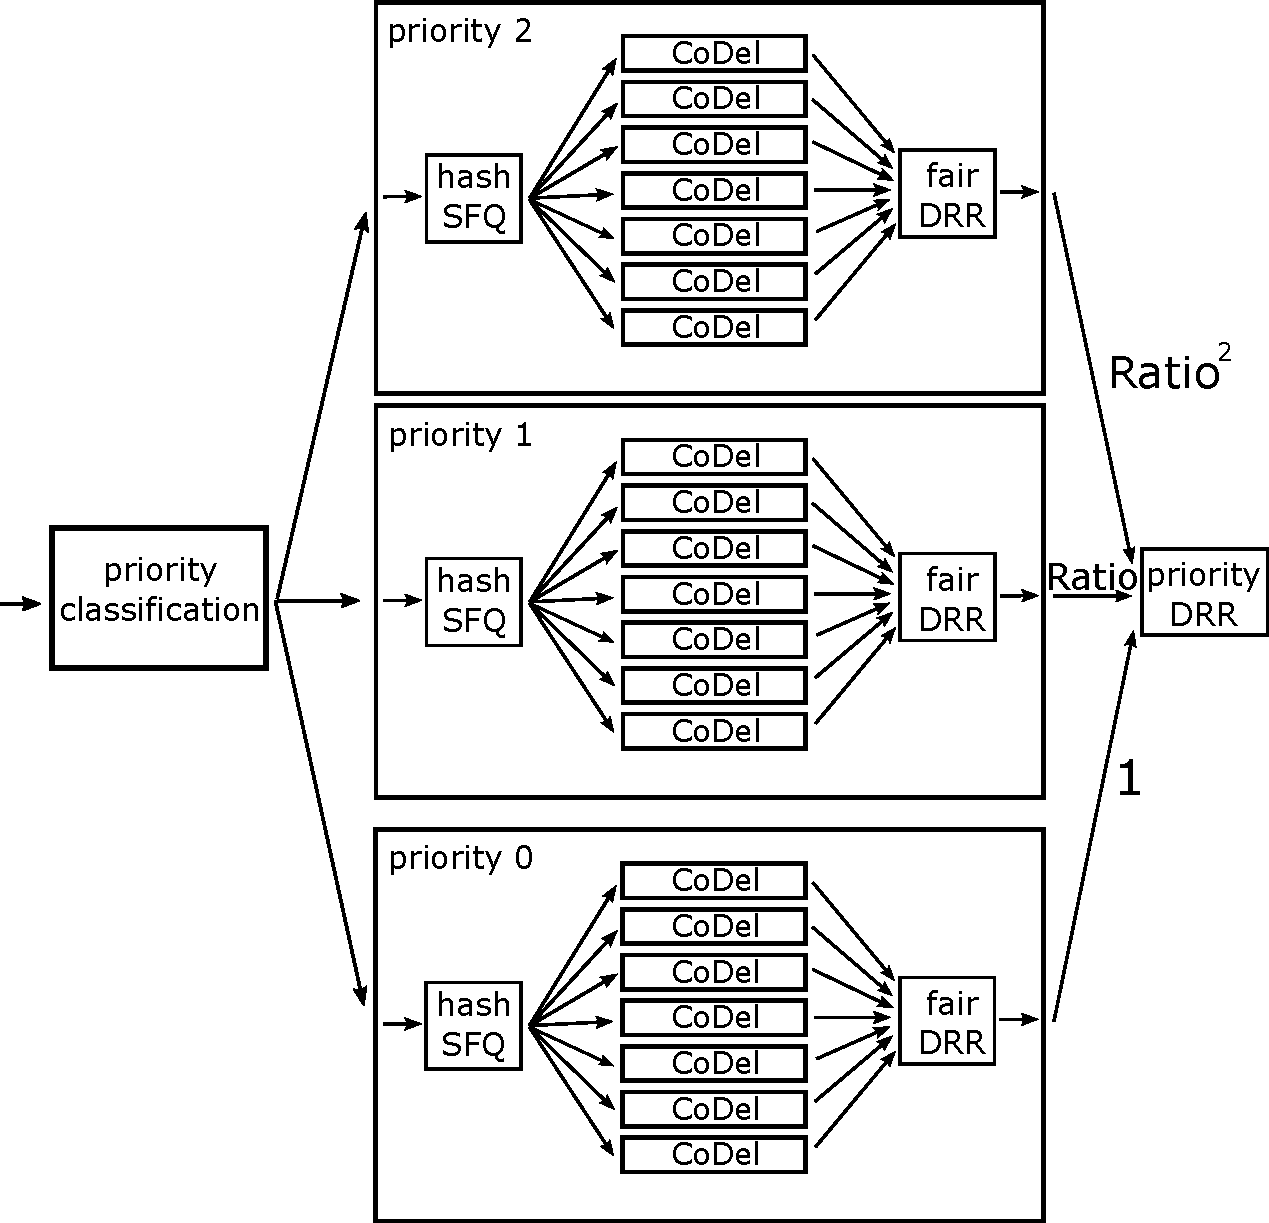
\includegraphics[width=137mm]{drawings/msfc}
	\caption{The MSFC layout}
	\label{fig10:msfc}
\end{figure}

In this thesis, we propose a traffic scheduler Multilevel stochastic fairness queueing (MSFC) illustrated in \ref{fig10:msfc}. It combines ideas of previous work: CoDel and deficit round-robin, to create class-aware traffic scheduler. It uses three-level layout. In the highest level, packets are assigned to priority classes. We use non-fair DRR to prioritize more important traffic. Inside the classes, packets are distributed into flows (based on source and destination IP addresses, ports and protocol) and we use second, independent fair DRR to schedule traffic within the class. Each flow uses CoDel algorithm.

MSFC takes $Ratio$ parameter. It defines the ratio of amount of resources between two adjacent priority classes. The amount of traffic rises exponentially: 


skombinovanie CoDel + SFQ + DRR + QoS


